\section{Travailler avec des données OGC}

% when the revision of a section has been finalized, 
% comment out the following line:
%\updatedisclaimer

% QGIS supports WMS and WFS as data sources. The support is native; WFS is
% implemented as a plugin.
QGIS gère le WMS et le WFS comme source de données. Leur gestion est native, mais
le service WFS  est géré sous forme d'extension.

% \subsection{What is OGC Data}\index{OGC!introduction}
\subsection{Qu'est ce que les données OGC}\index{OGC!introduction}

% The Open Geospatial Consortium (OGC), is an international organization with
more than 300 
% commercial, governmental, nonprofit and research organisations worldwide. Its
members 
% develop and implement standards for geospatial content and services, GIS data
processing 
% and exchange.
Le Consortium Geospatial Ouvert (Open Geospatial Consortium - OGC) est une
organisation internationale à laquelle participent plus de 300 organisations
commerciale, gouvernementale, associative et laboratoire de recherche à travers 
le monde. Ses membres développent et implémentent des standards pour les 
services et le contenu géospatial, traitement de données SIG et de format 
d'échange.

% Describing a basic data model for geographic features an increasing number of
specifications 
% are developed to serve specific needs for interoperable location and
geospatial technology, 
% including GIS. Further information can be found under
\url{http://www.opengeospatial.org/}.
%%An increasing number of specifications describing a basic data model for
%%geographic features are developed to serve specific needs for
%%interoperable location and geospatial technology,  including GIS.
Un nombre croissant de spécifications décrivant une modélisation de donnée
basique pour les objets géographiques ont été développées pour servir des besoins
spécifiques dans des situations nécessitant une interopérabilité et des technologies géospatiales,
dont les SIG. Des informations supplémentaires peuvent être trouvées sur le site
\url{http://www.opengeospatial.org/}.

% Important OGC specifications are:
Les spécifications importantes de l'OGC sont :

\begin{itemize}
\item \textbf{WMS} - Web Map Service
\item \textbf{WFS} - Web Feature Service
\item \textbf{WCS} - Web Coverage Service
\item \textbf{CAT} - Web Catalog Service
\item \textbf{SFS} - Simple Features for SQL
\item \textbf{GML} - Geography Markup Language
\end{itemize}

% OGC services are increasingly being used to exchange geospatial data between
% different GIS implementations and data stores. QGIS can now deal with three of
% the above specifications, being SFS (though support of the PostgreSQL /
PostGIS
% data provider, see Section \ref{label_postgis}); WFS and WMS as a client.
Les services OGC sont de plus en plus utilisés pour échanger des données
géospatiales entre différentes implémentations SIG et des fournisseurs de
données. QGIS peut maintenant traiter trois des spécifications citées, ceux-ci
étant SFS (par la gestion du fournisseur de données PostgreSQL / PostGIS, voir
section \ref{label_postgis}) ; comme client WFS et WMS.

\subsection{Client
WMS}\label{sec:ogc-wms}\index{WMS!client}\index{OGC!WMS!client}\index{
rasters!WMS}

\subsubsection{Aperçu de la gestion
WMS}\label{sec:ogc-wms-about}\index{WMS!client!about}

% QGIS currently can act as a WMS client that understands WMS 1.1, 1.1.1 and 1.3
% servers.  It has particularly been tested against publicly accessible servers
% such as DEMIS and JPL OnEarth.
QGIS peut actuellement agir comme client WMS et comprend les versions 1.1, 1.1.1
et 1.3 des serveurs WMS. Il a été particulièrement testé avec des serveurs
accessibles publiquement comme ceux de DEMIS et JPL OnEarth.

% WMS servers act upon requests by the client (e.g. QGIS) for a raster map with
% a given extent, set of layers, symbolisation style, and transparency.  The WMS
% server then consults its local data sources, rasterizes the map, and sends
% it back to the client in a raster format.  For QGIS this would typically
% be JPEG or PNG.
Les serveurs WMS agissent en fonction des requêtes envoyées par le client (par
exemple QGIS) pour une carte raster avec une étendue donnée, un ensemble de
couches, une sémiologie et une transparence. Le serveur WMS consulte alors ses
sources de données locales, rasterise la carte et la renvoie au client dans un
format raster. Pour QGIS cela sera par exemple du JPEG ou du PNG.

% WMS is generically a REST (Representational State Transfer) service rather
% than a fully-blown Web Service.  As such, you can actually take the URLs
% generated by QGIS and use them in a web browser to retrieve the same images
% that QGIS uses internally.  This can be useful for troubleshooting, as there
% are several brands of WMS servers in the market and they all have their own
% interpretation of the WMS standard.
Un WMS est de manière générale un service web mis en oeuvre selon une 
architecture REST (Representational State Transfer) plutôt qu'un service 
  RPC (Remote Procedure Call) pleinement déployé

% WMS layers can be added quite simply, as long as you know the URL to access
% the WMS server, you have a serviceable connection to that server, and the
% server understands HTTP as the data transport mechanism.
Des couches WMS peuvent être ajoutées assez simplement, du moment que vous
connaissez l'URL pour accéder au serveur WMS, vous avez une connexion sous
forme de service sur ce serveur, et celui-ci comprend le protocole HTTP comme
mécanisme de transport.

\subsubsection{Sélectionner des serveurs
WMS}\label{sec:ogc-wms-servers}\index{WMS!remote server!selection}

% The first time you use the WMS feature, there are no servers defined. You 
% can begin by clicking the \toolbtntwo{mActionAddWmsLayer}{Add WMS layer}
% button inside the toolbar, or through the
% \mainmenuopt{Layer}>\dropmenuopttwo{mActionAddWmsLayer}{Add WMS Layer...}
% menu.
La première fois que vous utilisez la fonctionnalité des services WMS, il y a
aucun serveur définie. Vous pouvez commencer en cliquant sur le bouton
\toolbtntwo{mActionAddWmsLayer}{Ajoutez une couche WMS} dans la barre des
outils ou à travers le menu
\mainmenuopt{Couche}>\dropmenuopttwo{mActionAddWmsLayer}{Ajoutez une couche
WMS...}

% The dialog \dialog{Add Layer(s) from a Server} for adding layers from the WMS
% server pops up. Fortunately you can add some servers to play with by clicking
% the \button{Add default servers} button. This will add at least three WMS
% servers for you to use, including the NASA (JPL) 
% WMS server. To define a new WMS server in the \tab{Server Connections}
% section, select \button{New}. Then enter in the parameters to connect to your
% desired WMS server, as listed in table \ref{tab:wms_connection_parms}:
La boîte de dialogue \dialog{Ajoute une couche d'un serveur} pour ajouter des
couches d'un serveur WMS s'ouvre. Heureusement, vous pouvez ajouter des
serveurs pour jouer en cliquant le bouton \button{Ajouter les serveurs par
défaut}. Cela ajoutera au moins trois serveurs WMS pour tester, incluant celui
de la NASA (JPL). Pour définir un nouveau serveur WMS dans la section
\tab{Connexions au serveur}, sélectionnez \button{Nouveau}. Puis entrez les
paramètres de connection de votre serveur WMS désiré, comme listé dans le
tableau \ref{tab:wms_connection_parms}:

\begin{table}[ht]\index{WMS!client!connection parameters}
\centering
% \caption{WMS Connection Parameters}\label{tab:wms_connection_parms}\medskip
\caption{Paramètres de connection WMS}\label{tab:wms_connection_parms}\medskip
 \begin{tabular}{|l|p{5in}|}
% \hline Name & A name for this connection.  This name will be used in the
%  Server Connections drop-down box so that you can distinguish it from
%  other WMS Servers. \\
\hline Nom & Un nom pour cette connexion. Ce nom sera utilisé dans la liste
 déroulante des connexions aux serveurs afin que vous puissiez distinguer
des autres serveurs WMS. \\
% \hline URL \index{WMS!URL} & URL of the server providing the data.
%  This must be a resolvable host name; the same format as you would use 
%  to open a telnet connection or ping a host. \\
\hline URL \index{WMS!URL} & URL du serveur fournissant les données. Cela doit
être un nom d'hôte publique ; de même format que vous utilisez pour ouvrir une
connexion Telnet ou pinguer un hôte (ou dans un navigateur Internet). \\
\hline
\end{tabular}
\end{table}

% If you need to set up a proxy-server to be able to receive WMS-services
% from the internet, you can add your proxy-server in the options.
% Choose menu \mainmenuopt{Settings} > \dropmenuopttwo{mActionOptions}{Options}
% and click on the \tab{Proxy} tab. There you can add your proxy-settings 
% and enable them by setting the \checkbox{Use proxy for web access}.
Si vous devez configurer un serveur proxy pour pouvoir recevoir des services
WMS à partir d'Internet, vous pouvez ajouter votre serveur proxy dans les
options. Choisissez le menu \mainmenuopt{Préférences} >
\dropmenuopttwo{mActionOptions}{Options...} et cliquez sur l'onglet
\tab{Proxy}. Vous pouvez alors ajouter votre configuration du proxy et
l'activer en cochant la case \checkbox{Utiliser un proxy pour l'accès Internet}.

% Once the new WMS Server connection has been created, it will be 
% preserved for future QGIS sessions.
Une fois que la nouvelle connexion du serveur WMS a été créée, elle sera
sauvegardée pour les futures sessions de QGIS.

% \begin{Tip}[ht]\caption{\textsc{On WMS Server URLs}}
% \qgistip{Be sure, when entering in the WMS server URL, that you have
% the base URL.  For example, you shouldn't have fragments such as
% \usertext{request=GetCapabilities} or \usertext{version=1.0.0}
% in your URL.\index{WMS!serveur distant!URL}
\begin{Astuce}[ht]\caption{\textsc{À propos des URL des serveurs WMS}}
\qgistip{Assurez vous, lorsque vous entrez l'url du serveur WMS, d'avoir le
début de l'URL. Par exemple, vous ne devez pas avoir ce genre de paramètre 
\usertext{request=GetCapabilities} ou \usertext{version=1.0.0}
dans votre URL\index{WMS!serveur distant!URL}
}
\end{Astuce}

% Table \ref{tab:wms_example_urls} shows some example WMS URLs to get you
% started. These links were last checked in December 2006, but could change at
% any time:
Le tableau \ref{tab:wms_example_urls} montre quelques exemples d'url WMS
pour démarrer. Ces liens ont été vérifié en décembre 2006, mais peuvent
avoir changer :

%FIXME:  WMS URLs should be checked again and maybe extended in QGIS 

\begin{table}[ht]\index{WMS!serveur distant!URL!exemples}
\centering
\caption{Exemple d'URL WMS publique}\label{tab:wms_example_urls}\medskip
 \begin{tabular}{|l|l|}
\hline \textbf{Nom}        & \textbf{URL} \\
\hline Atlas du Canada      & http://atlas.gc.ca/cgi-bin/atlaswms\_en? \\
\hline DEMIS                & http://www2.demis.nl/wms/wms.asp?wms=WorldMap\& \\
\hline Geoscience Australia &
http://www.ga.gov.au/bin/getmap.pl?dataset=national \\
\hline NASA JPL OnEarth     & http://wms.jpl.nasa.gov/wms.cgi? \\
\hline Utilsiateurs QGIS &
http://qgis.org/cgi-bin/mapserv?map=/var/www/maps/main.map\& \\
\hline
\end{tabular}
\end{table}

% An exhaustive list of WMS servers can be found at \url{http://wms-sites.com}.
Une liste de serveurs WMS exhaustive peut être trouvé ici
\url{http://wms-sites.com}.

\subsubsection{Charger des
couches WMS}\label{sec:ogc-wms-layers}\index{WMS!client!couches}

% Once you have successfully filled in your parameters you can select the
% \button{Connect} button to retrieve the capabilities of the selected server. 
% This includes the Image encoding, Layers, Layer Styles, and Projections. 
% Since this is a network operation, the speed of the response depends on the
% quality of your network connection to the WMS server. While downloading data
% from the WMS server, the download progress is visualized in the left bottom of
% the WMS Plugin dialog.
Une fois que vous avez remplie correctement vos paramètres vous pouvez
sélectionner le bouton \button{Se connecter} pour récupèrer les possibilités du
serveur sélectionné. Cela inclut le format d'image, les couches, les styles des
couches et les projections. Puisque c'est une opération sur un réseau, la
vitesse de la réponse dépend de la qualité de votre connection réseau au
serveur WMS. Pendant le téléchargement des données du serveur WMS, la
progression du téléchargement est visualisé en bas à gauche de la boîte de
dialogue du plugin WMS.

% Your screen should now look a bit like Figure \ref{fig:connection_wms}, which
% shows the response provided by the NASA JPL OnEarth WMS server.
Votre écran doit ressembler un peu plus à la figure \ref{fig:connection_wms},
qui affiche la réponse fournit par le serveur WMS de la NASA JPL OnEarth.

\begin{figure}[ht]
  \begin{center}
%    \caption{Dialog for adding a WMS server, showing its available layers
   \caption{Dialogue pour ajouter un serveur WMS, en indiquant ses couches
disponibles
\nixcaption}\label{fig:connection_wms}
 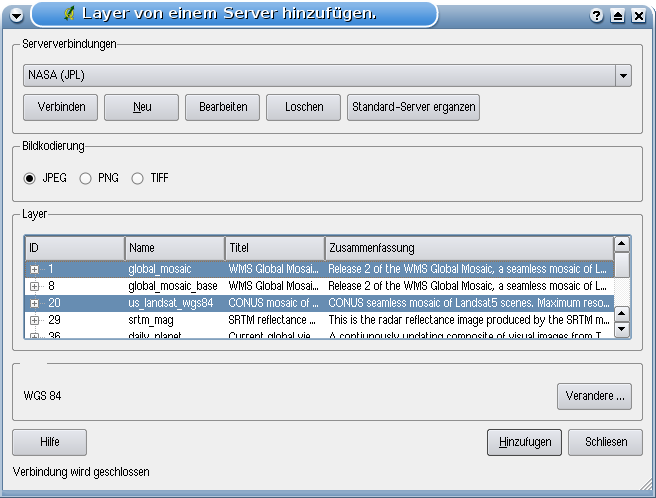
\includegraphics[clip=true,width=0.6\textwidth]{connection_wms}
  \end{center}
\end{figure}

% \minisec{Image Encoding}
\minisec{Format d'image}

% The \tab{Image encoding} section now lists the formats that are supported by
% both the client and server.  Choose one depending on your image accuracy
% requirements.
La section \tab{Format d'image} liste maintenant les formats qui sont gérés à
la fois par le client et leur serveur.Choisissez en un en fonction de votre
préférence quant à la précision de l'image.

% \begin{Tip}[ht]\caption{\textsc{Image Encoding}}
\begin{Astuce}[ht]\caption{\textsc{Format d'image}}

% \qgistip{You will typically find that a WMS server offers you the choice
% of JPEG or PNG image encoding.  JPEG is a lossy compression format,
% whereas PNG faithfully reproduces the raw raster data.
\qgistip{Les serveurs WMS vous offriront typiquement le choix entre les
formats d'image JPEG et PNG. JPEG est un format de compression avec perte,
tandis que le format PNG reproduit pleinenement les données raster brutes.

% Use JPEG if you expect the WMS data to be photographic in nature and/or you
% don't mind some loss in picture quality.  This trade-off typically reduces by
% 5 times the data transfer requirement compared to PNG.
Utilisez le format JPEG si vous pensez que la données WMS est une
orthophotographie ou qu'une perte de qualité d'image ne vous pose pas de
problème. Ce compromis vous permet de réduire par 5 le taux de transfert
nécessaire comparé au  format PNG.

% Use PNG if you want precise representations of the original data, and you
% don't mind the increased data transfer requirements.
Utilisez le format PNG si vous désirez une représentation précises des données
originales et que l'augmentation du taux de transfert ne vous pose pas de
problème.
\index{WMS!format d'image}
}
\end{Astuce}

\minisec{Couches}

% The \tab{Layers} section lists the layers available from the selected
% WMS server.  You may notice that some layers are expandible, this means
% that the layer can be displayed in a choice of image styles.
La section \tab{couche} liste les couches disponibles dans le serveur WMS. Vous
pouvez remarquer que certaines couches sont extensibles, cela signifie que la
couche peut être affiché en fonction de plusieurs styles.

% You can select several layers at once, but only one image style per layer.
% When several layers are selected, they will be combined at the WMS Server
% and transmitted to QGIS in one go.
Vous pouvez sélectionner plusieurs couches à la fois, mais seulement un style 
d'image par couche. Lorsque plusieurs couches sont sélectionnées, celles-ci 
seront combinées par le serveur WMS et transmises à QGIS en une seule fois.

% \begin{Tip}[ht]\caption{\textsc{WMS Layer Ordering}}
\begin{Astuce}[ht]\caption{\textsc{Ordonner les couches WMS}}
% \qgistip{In this version of QGIS, WMS layers rendered by a server are overlaid
% in the order listed in the Layers section, from top to bottom of the list.
% If you want to overlay layers in the opposite order, then you can 
% select \toolbtntwo{mActionAddWmsLayer}{Add WMS layer} a second time, choose 
% the same server again, and select the second group of layers that you want to 
% overlay the first group.\index{WMS!remote server!layer ordering}
\qgistip{Dans cette version de QGIS, les couches WMS créées par un serveur sont 
superposées dans l'ordre listé dans la section couches, du haut vers le bas de 
la liste. Si vous voulez superposer des couches dans l'ordre inverse, vous 
pouvez alors sélectionner \toolbtntwo{mActionAddWmsLayer}{Ajouter une couche 
WMS} une seconde fois, choisir le même serveur, et sélectionner un groupe de 
couches que vous voulez au-dessus du premier groupe.
\index{WMS!serveur distant!ordonner les couches}
}
\end{Astuce}

\minisec{Transparence}\label{ogc-wms-transparency}

% In this version of QGIS, the transparency setting is hard-coded to 
% be always on, where available.
Dans cette version de QGIS, le paramètre de transparence est codé en dur pour 
être toujours activé, si disponible.

% \begin{Tip}[ht]\caption{\textsc{WMS Layer Transparency}}
\begin{Astuce}[ht]\caption{\textsc{Transparence des couches WMS}}
% \qgistip{The availability of WMS image transparency depends on
% the image encoding used:  PNG and GIF support transparency,
% whilst JPEG leaves it unsupported.
% \index{WMS!transparence de couche}
% }
\qgistip{la disponibilité de la transparence de l'image WMS dépend du format
d'image utilisé : les formats PNG et GIF gère la transparence, tandis que le
format JPEG ne le gère pas. \index{WMS!transparence de couche}
}
\end{Astuce}

\minisec{Système de Référence de Coordonnées}
\index{WMS!CRS}\index{WMS!système de référence de coordonnées}
\index{OGC!CRS}\index{OGC!système de référence de coordonnées}
\index{Projections!WMS}
\index{Projections!CRS}\index{Projections!système de référence de coordonnées}
\index{CRS}\index{système de référence de coordonnées}
\index{SRS}\index{Projections!SRS}

% A Coordinate Reference System (CRS) is the OGC terminology for a QGIS
% Projection.
Un système de Référence de Coordonnées (CRS) est la terminologie de l'OGC pour
une projection QGIS.

% Each WMS Layer can be presented in multiple CRSs, depending on the capability
% of the WMS server.  You may notice that the \textsl{x} changes in the
% \textsl{Coordinate Reference System (x available)} header as you select and
% deselect layers from the \tab{Layers} section.
Chaque couche WMS peut être représenté dans plusieurs projections (ou CRS), en
fonction de la possibilité du serveur WMS. Vous pouvez avoir noté que les
\textsl{x} changent dans l'en-tête du \textsl{Système de Référence des
Coordonnées(x disponible)} lorsque vous sélectionnez et déselectionnez les
couches de la section \tab{couches}.

% To choose a CRS, select \button{Change...} and a screen similar to
% Figure \ref{fig:projections} in Section \ref{label_projstart} will appear.
% The main difference with the WMS version of the screen is that only
% those CRSs supported by the WMS Server will be shown.
Pour choisir une projection, sélectionnez \button{Changer...} et un écran
similaire à la figure \ref{fig:projections} dans la section
\ref{label_projstart} apparaitra. La principale différence avec l'écran de la
version WMS est que seules les projections gérées par le serveur sera listées.

% \begin{Tip}[ht]\caption{\textsc{WMS Projections}}
\begin{Astuce}[ht]\caption{\textsc{Les projections WMS}}
% \qgistip{For best results, make the WMS layer the first layer you add in the
% project.  This allows the project projection to inherit the CRS you used to
% render the WMS layer. On-the-fly projection (see
% Section \ref{sec:projection-specifying}) can then be used to fit any
% subsequent vector layers to the project projection. In this version of QGIS,
% if you add a WMS layer later, and give it a different CRS to the current
% project projection, unpredictable results can occur.}
\qgistip{Pour de meilleurs résultats, faîtes en sorte que la couche WMS soit la
première couche que vous ajoutez dans le projet. Cela permet à la projection du
projet d'hériter la définition de la projection que vous avez utilisé pour le
rendu de la couche WMS. La projection à la volée (voir Section
\ref{sec:projection-specifying}) peut être utilisée pour placer les couches
vectorielles supplémentaires dans la projection du projet. Dans cette version 
de QGIS, si vous ajoutez une couche WMS plus tard et lui donner une projection
différente de celui du projet en cours, cel apeut entraîner des résultats
aléatoires.}
\end{Astuce}


% \subsubsection{Using the Identify Tool}\label{sec:ogc-wms-identify}
\subsubsection{Utiliser l'outil Identifier}\label{sec:ogc-wms-identify}
\index{WMS!identifier}
\index{identifier!WMS}
\index{WMS!GetFeatureInfo}

% Once you have added a WMS server, and if any layer from a WMS server is
% queryable, you can then use the \toolbtntwo{mActionIdentify}{Identify} tool to
% select a pixel on the map canvas. A query is made to the WMS server for each
% selection made.
Une fois que vous avez ajouté un serveur WMS et si une couche du serveur WMS
est intérogeable, vous pouvez utiliser l'outil 
\toolbtntwo{mActionIdentify}{Identifier} pour sélectionner un pixel sur la
carte. Une requête est envoyée au serveur WMS pour chaque sélection effectuée.

% The results of the query are returned in plain text. The formatting of this
% text is dependent on the particular WMS server used.
Les résultats de la requête sont renvoyés au format texte. Le formattage de ce
texte est dépendant du serveur WMS utilisé.

% FIXME: GetFeatureInfo-Requests are done here?

% \subsubsection{Viewing Properties}
\subsubsection{Visualiser les propriétés}
\label{sec:ogc-wms-properties}\index{WMS!propriétés}
\index{rasters!propriétés}

% Once you have added a WMS server, you can view its properties by
% right-clicking on it in the legend, and selecting \button{Properties}.
Une fois que vous avez ajouté un serveur WMS, vous pouvez voir ses propriétés
en cliquant avec le bouton droit de la souris sur sa légende, et en
sélectionnant le bouton  \button{Propriétés}.

% \minisec{Metadata Tab}\label{sec:ogc-wms-properties-metadata}
\minisec{Onglet métadonnées}\label{sec:ogc-wms-properties-metadata}
\index{rasters!métadonnées}
\index{WMS!métadonnées}
\index{WMS!possibilités}

% The \tab{Metadata} tab displays a wealth of information about the WMS server,
% generally collected from the Capabilities statement returned from that server.
L'onglet \tab{métadonnées} affiche la richesse des informations du serveur WMS,
généralement collecté à partir de la requête Capabilities renvoyée par le
serveur.

% Many definitions can be gleaned by reading the WMS standards
% \cite{OGCWMS010101web}, \cite{OGCWMS010300web}, but here are a few handy
% definitions:
Beaucoup de définitions peuvent être obtenues par la lecture des normes WMS
\cite{OGCWMS010101web}, \cite{OGCWMS010300web}, mais en voici quelques-unes :

\begin{itemize}
% \item \textbf{Server Properties}
\item \textbf{Propriétés du serveur}

\begin{itemize}
% \item \textbf{WMS Version}      - The WMS version supported by the server.
\item \textbf{Version du WMS}      - la version du serveur WMS géré par le
serveur.

% \item \textbf{Image Formats}    - The list of MIME-types the server can
% respond with when drawing the map.  QGIS supports whatever formats the
% underlying Qt libraries were built with, which is typically at least
% \texttt{image/png} and \texttt{image/jpeg}.
\item \textbf{Formats d'image}    - la liste des types MIME que le serveur peut
renvoyer lors qu'il dessinne la carte. QGIS gère tous les formats pour
lesquelles la bibliothèque Qt en sous-couche a été compilée, qui est
typiquement à minima les types \texttt{image/png} et \texttt{image/jpeg}.

% \item \textbf{Identity Formats} - The list of MIME-types the server can
% respond with when you use the Identify tool.  Currently QGIS supports the
% \texttt{text-plain} type.
\item \textbf{Formats de l'outil Identitier} - la liste des types
MIME auxquels le serveur peut répondre quand vous utilisez l'outil
Identifier. Pour l'instant QGIS gère le type \texttt{text-plain}.
\end{itemize}

% \item \textbf{Layer Properties}
\item \textbf{Propriétés de la couche}

\begin{itemize}
% \item \textbf{Selected}         - Whether or not this layer was selected when
% its server was added to this project.
\item \textbf{Selectioné}         - si cette couche a été sélectionnée ou pas
quand son serveur a été ajouté au projet.

% \item \textbf{Visible}          - Whether or not this layer is selected as
% visible in the legend.  (Not yet used in this version of QGIS.)
\item \textbf{Visible}          - si cette couche a été sélectionnée ou non
comme visible dans la légende (pas encore utilisé dans cette version de QGIS).

% \item \textbf{Can Identify}     - Whether or not this layer will return any
% results when the Identify tool is used on it.
\item \textbf{Peut identifier}     - si cette couche retournera ou pas des
résultats quand l'outil Identifier est utilisé sur celle-ci.

% \item \textbf{Can be Transparent} - Whether or not this layer can be rendered
% with transparency. This version of QGIS will always use transparency if this
is
% \textsl{Yes} and the image encoding supports transparency
\item \textbf{Peut être transparent} - si cette couche peut être rendu ou
non avec une transparence. Cette version de QGIS utilisera toujours la
transparence si cette option est à \textsl{Oui} et que le format d'image gère
la transparence
% BM: doesn't seem to work?
%                                    (see Section
%                                    \ref{ogc-wms-transparency}
%                                    ).
                                    .

% \item \textbf{Can Zoom In}      - Whether or not this layer can be zoomed in
% by the server.  This version of QGIS assumes all WMS layers have this set
% to \textsl{Yes}. Deficient layers may be rendered strangely.
\item \textbf{Peut zoomer}      - si on peut zoomer ou non sur cette couche
avec le serveur. Cette version de QGIS assume que toutes les couches WMS ont ce
paramètre définie à \textsl{Oui}. Les couches déficientes peuvent être rendu
d'une manière étrange.

% \item \textbf{Cascade Count}    - WMS servers can act as a proxy to other WMS
% servers to get the raster data for a layer.  This entry shows
% how many times the request for this layer is forwarded to peer WMS servers for
% a result.
\item \textbf{décompte des cascades}    - les serveurs WMS peuvent agir comme
un proxy à d'autres serveurs WMS pour obtenir des données pour une couche.
Cette entrée affiche combien de fois la requête pour cette couche est
redirigée vers un autre serveur WMS pour un résultat.

% \item \textbf{Fixed Width}, \textbf{Fixed Height}     - Whether or not this
% layer has fixed source pixel dimensions. This version of QGIS assumes all WMS
% layers have this set to nothing. Deficient layers may be rendered strangely.
\item \textbf{Largeur fixe}, \textbf{hauteur fixe}     - si une couche a
des dimensions du pixel source limitées. Cette version de QGIs suppose que
toutes les couches WMS ont ce paramètre fixé. Les couches déficientes  peuvent
être rendu d'une manière étrange.

% \item \textbf{WGS 84 Bounding Box} - The bounding box of the layer, in WGS 84
% coordinates. Some WMS servers do not set this correctly (e.g. UTM coordinates
% are used instead).  If this is the case, then the initial view of this layer
% may be rendered with a very ``zoomed-out'' appearance by QGIS. The WMS
% webmaster should be informed of this error, which they may know as the WMS XML
% elements \texttt{LatLonBoundingBox}, \texttt{EX\_GeographicBoundingBox} or the
% CRS:84 \texttt{BoundingBox}.
\item \textbf{Limite du contour en WGS 84} - la limite du contour de la
couche, en coordonnées WGS 84. Certains serveurs WMS ne définissent pas ceci
correctement (par exemple des coordonnées UTM sont utilisées à la place). Si
cela est le cas, alors la vue initiale sera rendu avec une vue très étendue. Le
webmaster du WMS doit être informé de cette erreur, qui sont connu en tant
qu'éléments XML \texttt{LatLonBoundingBox}, \texttt{EX\_GeographicBoundingBox}
ou \texttt{BoundingBox} CRS:84 du WMS.

% \item \textbf{Available in CRS} - The projections that this layer can be
% rendered in by the WMS server. These are listed in the WMS-native format.
\item \textbf{Disponibilité des CRS} - les projections que l'on peut utiliser
par le serveur WMS. Ceux-ci sont listés dans le format natif du WMS.

% \item \textbf{Available in style} - The image styles that this layer can be
% rendered in by the WMS server.
\item \textbf{Disponibilité des styles} - les styles des images de cette couche
qui peuvent être utilisé pour le rendu par le serveur WMS.

\end{itemize}

\end{itemize}


% \subsubsection{WMS Client
% Limitations}\label{sec:ogc-wms-limits}\index{WMS!client!limits}
\subsubsection{Limitations du client
WMS}\label{sec:ogc-wms-limits}\index{WMS!client!limites}

% Not all possible WMS Client functionality had been included in this version of
% QGIS. Some of the more notable exceptions follow:
Seule quelques fonctionnalités du client WMS ont été incluses dans cette
version de QGIS. Les exceptions les plus notables sont présentées ci-après :

% \minisec{Editing WMS Layer Settings}
\minisec{Éditer la configuration d'une couche WMS}
\index{WMS!configuration des couches!édition}

% Once you've completed the \toolbtntwo{mActionAddWmsLayer}{Add WMS layer}
% procedure, there is no ability to change the settings.
Une fois que vous avez complété la procédure d'
\toolbtntwo{mActionAddWmsLayer}{Ajout de couches WMS}, il n'y aucun moyen
de modifier la configuration.

% A workaround is to delete the layer completely and start again.
Une solution de contournement est de supprimer la couche et de recommencer.

% \minisec{WMS Servers Requiring Authentication}
\minisec{Serveurs WMS nécessitant une authentification}
\index{WMS!serveur distant!authentication}

% Only public WMS servers are accessible.
% There is no ability to apply a user name and password combination
% as an authentication to the WMS server.
Seuls les serveurs WMS public sont accessibles.
Il n'y a pas de possibilité pour appliquer une combinaison nom d'utilisateur
et mot de passe comme authentification à un serveur WMS.

% \begin{Tip}[ht]\caption{\textsc{Accessing secured OGC-layers}}
\begin{Astuce}[ht]\caption{\textsc{Accéder des couches OGC sécurisées}}
% \qgistip{If you need to access secured layers, you could use InteProxy as
% a transparent proxy, which does supports several authentification methods.
% More information can be found at the InteProxy-manual found on the website
% \url{http://inteproxy.wald.intevation.org}.
\qgistip{Si vous avez besoin d'accéder à des couches sécurisées, vous pouvez
utiliser InteProxy comme proxy transparent, qui gère plusieurs méthodes
d'authentification. Vous pouvez trouver plus d'informations dans le manuel
InteProxy que vous pouvez trouver sur le
site \url{http://inteproxy.wald.intevation.org}.
\index{WMS!couches sécurisées!}\index{OGC!Authentication}
}
\end{Astuce}


% \subsection{WFS Client}
\subsection{Client WFS}

% In QGIS, a WFS layer behaves pretty much like any other vector layer. You 
% can identify and select features and view the attribute table. An exception 
% is that editing is not supported at this time. To start the WFS plugin you 
% need to open \mainmenuopt{Plugins} >
% \dropmenuopttwo{mActionShowPluginManager}{Plugin Manager...}, 
% activate the \checkbox{WFS plugin} checkbox and click \button{OK}.
Dans QGIS, une couche WFS se comporte à peu près comme n'importe quelle autre
couche vecteur. Vous pouvez identifier et sélectionner des objets et
voir la table attributaire. Une exception est que l'édition n'est
pas prise en charge pour l'instant. Pour lancer le plugin WFS, vous avez besoin
d'ouvrir des \mainmenuopt{Plugins} >
\dropmenuopttwo{mActionShowPluginManager}{Gestionnaire de plugin ...}, activez
le \checkbox{plugin WFS} et cliquez sur le bouton \button{OK}.

% A new \toolbtntwo{mIconAddWfsLayer}{Add WFS Layer} icon appears next 
% to the WMS icon. Click on it to open the dialog. In General adding a WFS 
% layer is very similar to the procedure used with WMS. The difference is 
% there are no default servers defined, so we have to add our own.
Une nouvelle icône \toolbtntwo{mIconAddWfsLayer.png}{Ajouter une couche WFS}
apparaît à côté de celle du WMS. Cliquez dessus pour ouvrir la boîte de
dialogue. En général ajouter une couche WFS est identique à la procédure
utilisée pour une couche WMS. La différence est qu'il n'y a pas de serveurs par
défaut, vous devez donc en ajouter.

% \subsubsection{Loading a WFS Layer}
\subsubsection{Charger une couche WFS}

% As an example we use the DM Solutions WFS server and display a layer. The URL
% is:
Comme exemple, nous utilisons le serveur WFS de DM Solutions et affichons une
couche. L'url est :
\begin{verbatim}
http://www2.dmsolutions.ca/cgi-bin/mswfs_gmap?VERSION=1.0.0&SERVICE=
wfs&REQUEST=GetCapabilities
\end{verbatim}

\begin{enumerate}
%   \item Make sure the WFS plugin is loaded; if not, open the Plugin Manager and
% load it
  \item Assurez vous que le plugin WFS est activée ; Si ce n'est pas le cas,
ouvrez le gestionnaire de plugin et activez le.
%   \item Click on the \toolbtntwo{mIconAddWfsLayer}{Add WFS Layer} tool on the
% plugins toolbar
  \item Cliquez sur le bouton \toolbtntwo{mIconAddWfsLayer}{Ajoutez une couche
WFS} dans la boîte à outil des plugins.
%   \item Click on \button{New} 
  \item Cliquez sur \button{Nouveau} 
%   \item Enter \inputtext{Name}{DM Solutions} as the name
  \item Entrez \inputtext{Nom}{DM Solutions} comme nom.
%   \item Enter the URL (see previous page)
\item Entrez l'url (voir page précédente).
%   \item Click \button{OK}
\item Cliquez sur \button{OK}
%   \item Choose \selectstring{Server Connections}{DM Solutions} from the
% drop-down box
  \item Choisissez \selectstring{Connections au serveur}{DM Solutions} dans la
liste déroulante.
%   \item Click \button{Connect}
\item Cliquez sur \button{Connect}.
%   \item Wait for the list of layers to be populated
\item Attendez que la liste des couches soit complètes.
%   \item Click on the \clicklistitem{Canadian Land} layer
\item Cliquez sur la couche\clicklistitem{Canadian Land}.
%   \item Click \button{Add} to add the layer to the map
\item Cliquez sur \button{Ajoutez} pour ajouter la couche à la carte.
%   \item Wait patiently for the features to appear
\item Patientez que les objets apparaissent.
\end{enumerate}

\begin{figure}[ht]
  \begin{center}
%    \caption{Adding a WFS layer \nixcaption}\label{fig:wfs_dmsolutions}
 \caption{Ajoutez une couche WFS\nixcaption}\label{fig:wfs_dmsolutions}
 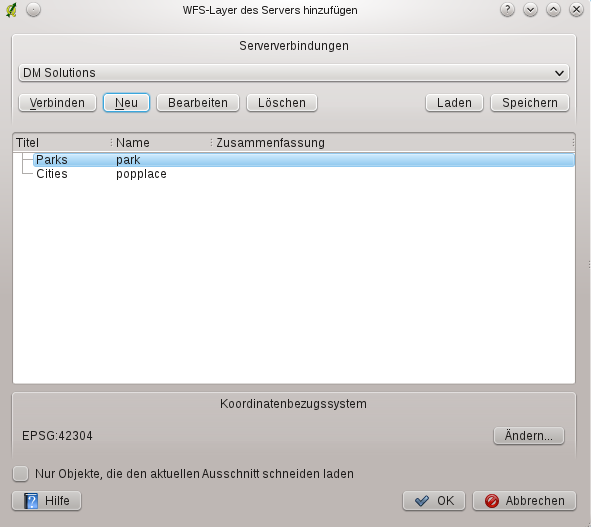
\includegraphics[clip=true,width=0.6\textwidth]{connection_wfs}
  \end{center}
\end{figure}
% You'll notice the download progress is visualized in the left bottom of the
% QGIS main window. 
% Once the layer is loaded, you can identify and select a province or two and
% view the attribute table.
Vous remarquerez que la progression du téléchargement est affichée en bas à
gauche de la fenêtre principale de QGIS.

% Remember this plugin works best with UMN MapServer WFS servers. It still
% could be, that you might experience random behavior and crashes. You can look
% forward to improvements in a future version of the plugin.
Souvenez vous que les plugins fonctionnent mieux avec des serveurs WFS sous
MapServer. Il est encore possible que vous ayez à faire face à quelques
problèmes et crashes. Vous pouvez vous attendre à des améliorations dans les
versions futures du plugin.

% \begin{Tip}[ht]\caption{\textsc{Finding WMS and WFS Servers}}
\begin{Astuce}[ht]\caption{\textsc{Trouver des serveurs WMS et WFS}}
% \qgistip{You can find additional WMS and WFS servers by using Google or your
% favorite search engine. There are a number of lists with public URLs, some 
% of them maintained and some not.
\qgistip{Vous pouvez trouver des serveurs WMS et WFS supplémentaire en utilisant
Google ou votre moteur de recherche préféré. Il y a un certain nombre de site
qui liste des url publiques, certaines maintenues d'autres non.
\index{WFS!serveur distant!}
}
\end{Astuce}